%!TEX root = ..\main.tex
\section{Model}

We consider colloidal particles with a permanent dipole moment $\mu \hat{m}$, where $\hat{m}$ is is a unitary vector with the direction of the dipole moment. While considering a three-dimensional system, we constrain particle movements to a one-dimensional line, i.e. particles are confined to the $z$ axis. However, particles can explore the full three dimensional orientation space. \textcolor{red}{um, I thougth that $z$ axis is a definition in itself? Just in case, how do I define it?}

The particle-particle interaction consists of two contributions: a dipole-dipole interaction and a short-range repulsion.

The energy of dipole-dipole interaction is given by

\label{eq:dipole_dipole_interaction}
\begin{equation}
E^{dip}_{12} = - \frac{\mu_1 \mu_2}{\Delta r^3}[3 (\hat{m}_1 \cdot \hat{r}_{12})(\hat{m}_2 \cdot \hat{r}_{12}) - (\hat{m}_1 \cdot \hat{m}_2)]
\end{equation}
where $\mu_1 \hat{m}_1$ and $\mu_2 \hat{m}_2$ are dipole moments of interacting particles, $\vec{r}_{12}$ is the direction vector which connects particle centers, whereas $\Delta r$ stands for the distance between particle centers.

By constraining particles in 1D tube we effectively enforce $\vec{r}_{12}$ to be co-aligned with $z$ axis. Defining energy in the units of particle dipole moment and assuming that all particles have the same dipole moment, (\ref{eq:dipole_dipole_interaction}) can be simplified in the following way:

\label{eq_dipole_dipole_1D}
\begin{equation}
E_{12}^{dip} = - \frac{1}{\Delta z^3} [3 \cos \theta_1 \cos \theta_2 - (\hat{m}_1 \cdot \hat{m}_2)]
\end{equation}
where $\theta_1$ and $\theta_2$ are the angles between $z$ axis and dipole moments of the first and second particle respectfully, and $\Delta z = |z_2 - z_1|$, where $z_1$ and $z_2$ are displacements of particle centers along $z$ axis. Because of three-dimensionality of our model, we can't simplify the last term, which accounts for relative orientation of the particles.

The repulsive part is described by Yukawa potential
\label{eq_yukawa_interaction}
\begin{equation}
E_{12}^{rep} = \frac{A \exp(-k \Delta z)}{\Delta z}
\end{equation}
Summarizing all of the above, the particle-particle interaction potential is presented in the following form:
\label{eq:full_particle_particle_interraction}
\begin{equation}
E_{12} = \left\{ \frac{A \exp(-k \Delta z)}{\Delta z} -  \frac{1}{\Delta z^3} [3 \cos \theta_1 \cos \theta_2 - (\hat{m}_1 \cdot \hat{m}_2)]\right\}
\end{equation}
where $A$ and $k$ -- parameters which governs repulsion hardness and coupling energy. Figure \ref{fig:interaction_energy} show examples of $E_{12}$ for different parameters.

\begin{figure}[h]
\begin{subfigure}{\textwidth}
\begin{subfigure}{.5\textwidth}
	\centering
	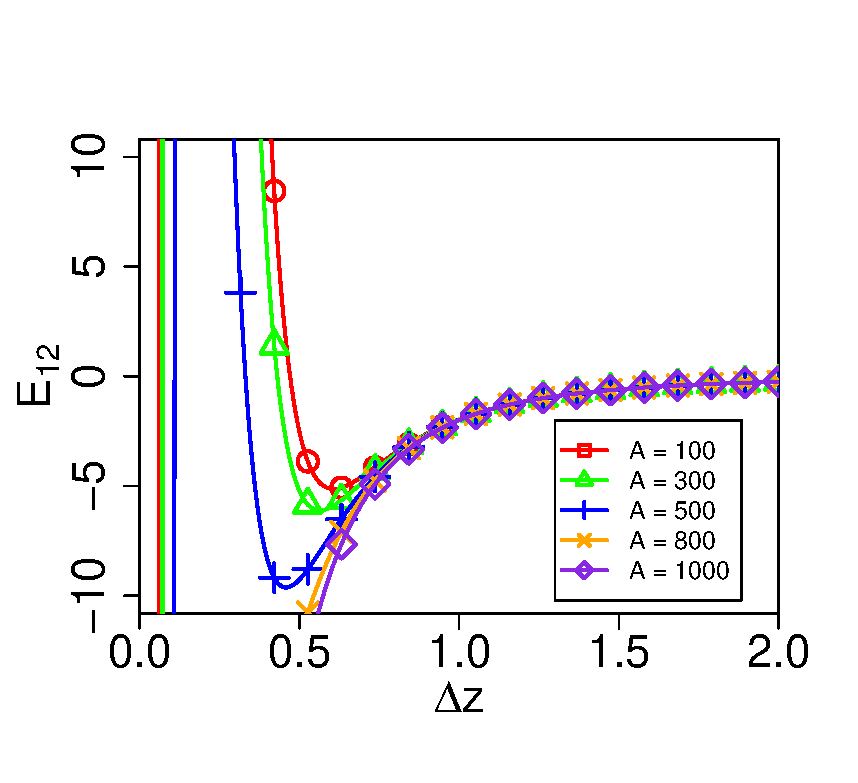
\includegraphics[width=\textwidth]{Images/k=10}
\end{subfigure}
\begin{subfigure}{.5\textwidth}
	\centering
	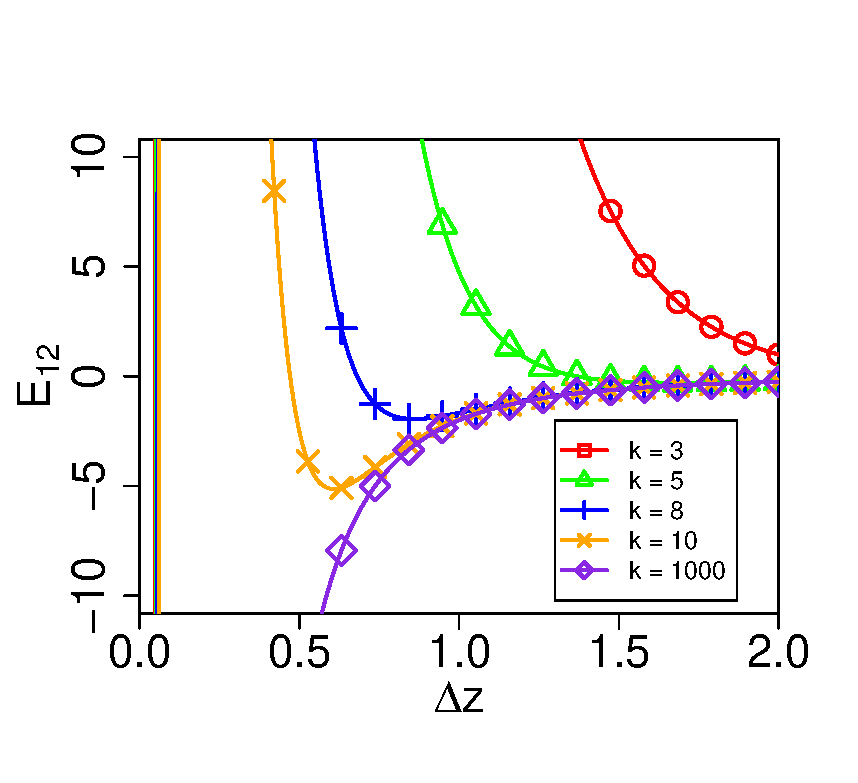
\includegraphics[width=\textwidth]{Images/A=1000}
\end{subfigure}
	\captionsetup{justification=centering, width=0.8\textwidth, singlelinecheck=false}
	\caption{Particles dipole moments are both co-aligned with $z$ axis}
    \label{fig:interaction_energy_coaligned}
\end{subfigure}

\begin{subfigure}{\textwidth}
\begin{subfigure}{.5\textwidth}
	\centering
	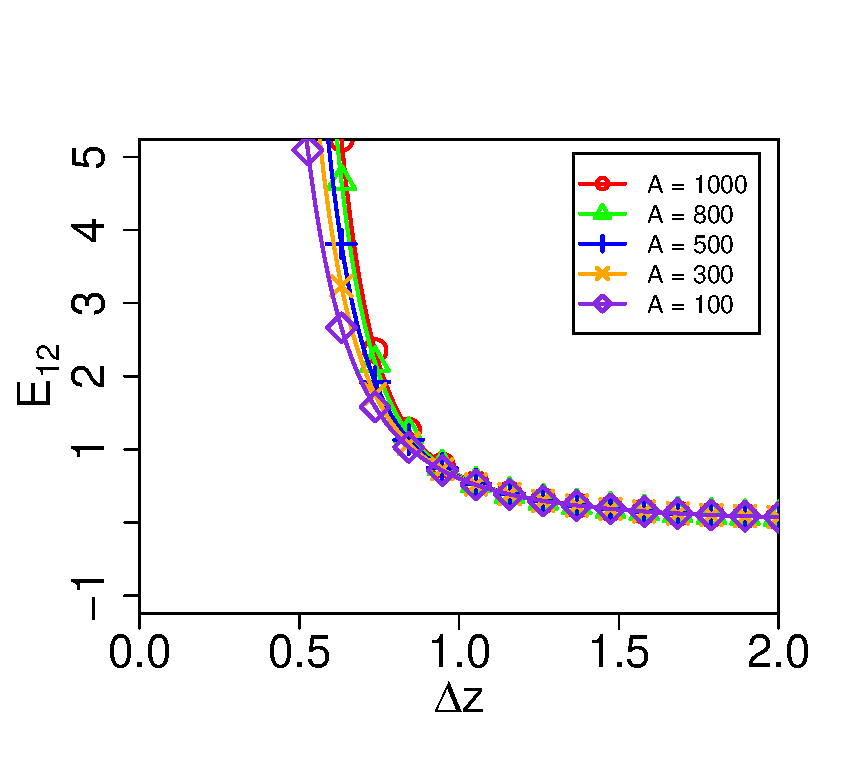
\includegraphics[width=\textwidth]{Images/k=10_perp}
\end{subfigure}
\begin{subfigure}{.5\textwidth}
	\centering
	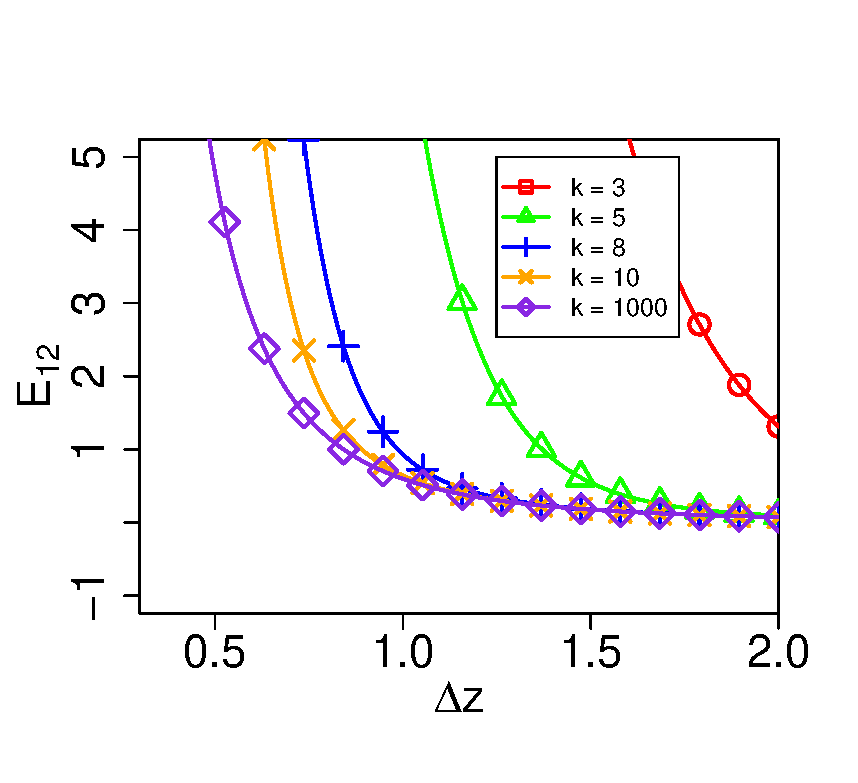
\includegraphics[width=\textwidth]{Images/A=1000_perp}
\end{subfigure}
	\captionsetup{justification=centering, width=0.8\textwidth, singlelinecheck=false}
	\caption{First particle dipole moment is co-aligned and second particle dipole moment is perpendicular to $z$ axis}
    \label{fig:interaction_energy_counteraligned}
\end{subfigure}
\captionsetup{justification=centering, width=0.9\textwidth}
\caption{Interaction energy as function of distance between centres of two interacting particles for co-aligned (\ref{fig:interaction_energy_coaligned}) and perpendicular (\ref{fig:interaction_energy_counteraligned}) orientation of the particles dipole moments. Left plots show energy for the fixed value of $k = 10$, and right for the fixed value of $A = 1000$}
\label{fig:interaction_energy}
\end{figure}

For the case when particles dipole moments are perpendicular to each other the interaction is purely repulsive. However, as we can see on the Figure \ref{fig:interaction_energy_coaligned}, for low values of $A$, combined with high values of $k$, we can observe purely attractive interaction. Since this produce physically uninteresting behaviour, we assumed $A = 1000$ and $k = 10$, the case where interaction energy have well-defined minimum and maximum.

%\begin{figure}[h]
%    \centering
%	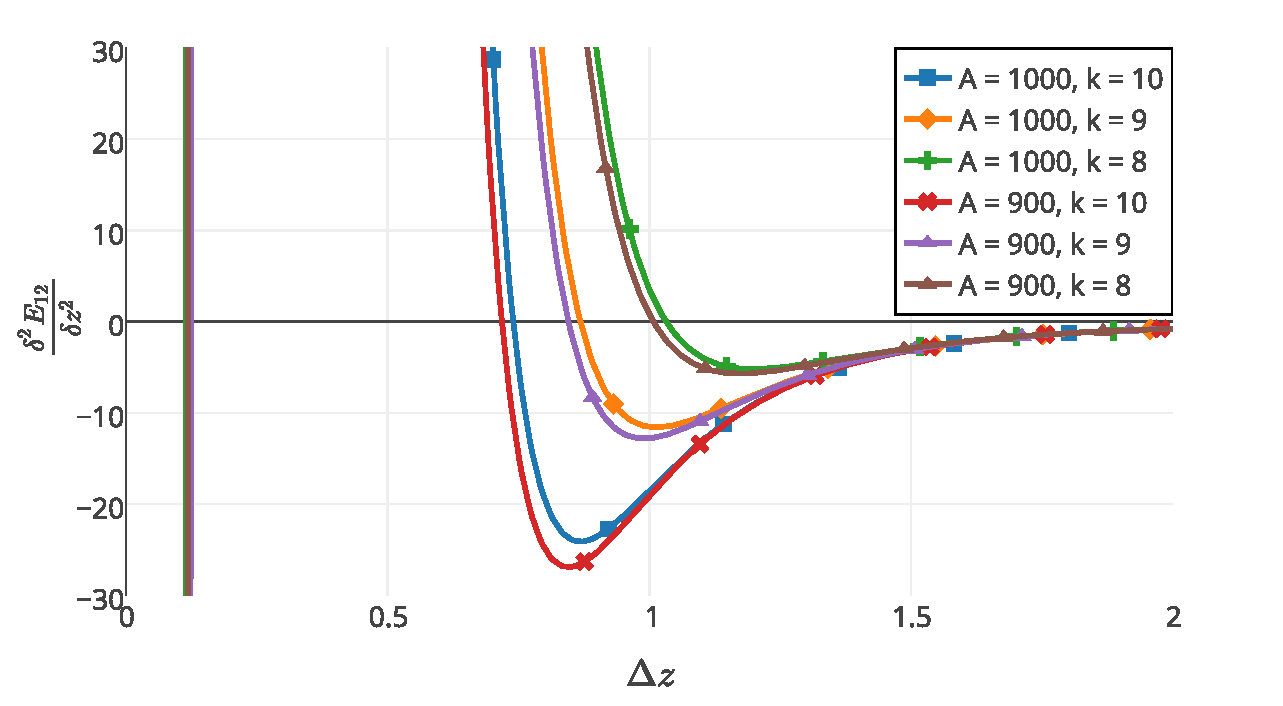
\includegraphics[width=.6\textwidth]{Energy_deriv2_r_difAK}
%	\captionsetup{justification=centering, width=0.8\textwidth}
%	\caption{Second derivative of interaction energy as function of distance between centres of two co-aligned particles ($\theta_1 = \theta_2 = 0$)}
%	\label{fig:energy_second_derivative}
%\end{figure}
